
\documentclass{standalone}

\usepackage{tikz}

\begin{document}

  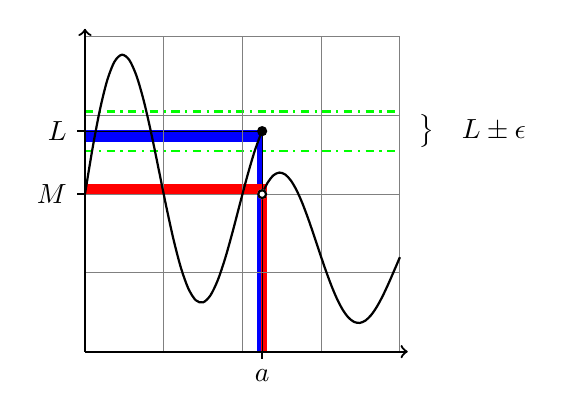
\begin{tikzpicture}[smooth,thick]
    \draw[color=green,dashdotted] (0,3.05)--(4,3.05);
    \draw[color=green,dashdotted] (0,2.55)--(4,2.55);
    \draw (4.1,2.8) node[right]{$\bigr\} \quad L \pm \epsilon$};
    \draw[fill,color=blue] (2.20,0) -- (2.2,2.68) -- (0,2.68) -- (0,2.8) -- (2.25,2.8) -- (2.25,0);
    \draw[fill,color=red] (2.3,0) -- (2.3,2.11) -- (0,2.11) -- (0,2) -- (2.25,2) -- (2.25,0);
    \draw[thin] (2.25,0) -- (2.25,2.8) -- (0,2.8);
    \draw[color=gray,thin] (0,0) grid (4,4);
    \draw[domain=0:2.25] plot (\x,{2+2*exp(-\x/4)*sin(pi*\x r)});
    \draw[domain=2.25:4] plot (\x,{1.2+2*exp(-\x/4)*sin(pi*\x r)});
    \draw[fill] (2.25,2.8) circle(.05);
    \draw[fill,color=white] (2.25,2) circle(.05);
    \draw (2.25,2) circle(.05);
    \draw[->] (0,0) -- (4.1,0);
    \draw (2.25,0)--(2.25,-.1) node[below]{$a$};
    \draw[->] (0,0) -- (0,4.1);
    \draw (0,2.8)--(-.1,2.8) node[left]{$L$};
    \draw (0,2)--(-.1,2) node[left]{$M$};
  \end{tikzpicture}

\end{document}
